\chapter{実装}
\label{implementation}

本章では提案手法の実装について述べる.

\section{拍認識の実装}
拍認識には様々な手法が存在する.

\section{演奏予測の実装}
演奏予測には様々な手法が存在する.
----- ここで過去の手法について紹介
今回は音楽的な表現の伝達に十分な精度しか必要ないため,/cite{tablenet}で用いられた手法を参考にした簡易的な予測手法を用いる.

\begin{figure}[htbp]
  \centering
  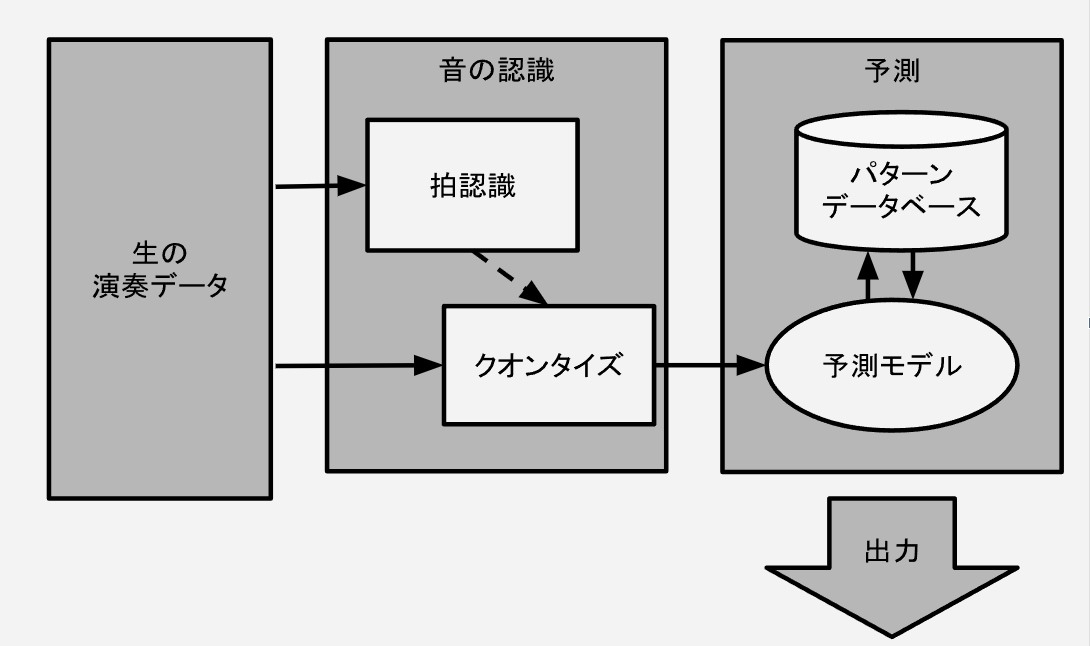
\includegraphics[width=0.8\linewidth]{src/pred.png}
  \caption{本システムの予測システム}
  \label{fig:tablenet}
\end{figure}

\section{位相修正}
受信部分において演奏相手の演奏予測を受け取った際,遅延を考慮して位相をずらして再生する必要がある.

%%% Local Variables:
%%% mode: japanese-latex
%%% TeX-master: "../bthesis"
%%% End:
